\documentclass[11pt]{article}
\usepackage[a4paper,margin=1in]{geometry}
\usepackage{amsmath,amssymb,amsfonts}
\usepackage{graphicx}
\usepackage{booktabs}
\usepackage{siunitx}
\usepackage{xcolor}
\usepackage{enumitem}
\usepackage[colorlinks=true,linkcolor=blue,citecolor=blue,urlcolor=blue]{hyperref}
\usepackage{caption}
\captionsetup{font=small,labelfont=bf}

\newcommand{\eps}{\varepsilon}
\newcommand{\vecr}{\mathbf{r}}
\newcommand{\vecE}{\mathbf{E}}
\newcommand{\Om}{\hat{\boldsymbol{\Omega}}}
\newcommand{\gradr}{\nabla_{\!\vecr}}
\newcommand{\honest}[1]{\par\medskip\noindent{\setlength{\fboxsep}{7pt}%
\colorbox{yellow!22}{\begin{minipage}{\dimexpr\linewidth-2\fboxsep\relax}%
\small\textbf{Honesty note.} #1\end{minipage}}}\par\medskip}

\title{\textbf{Numerical Reproduction of Liang, Goldsman, Mayergoyz \& Oldiges (1997):\\
2-D Deterministic SHE-Boltzmann MOSFET Simulation}\\[4pt]
\large\textit{Part~II (Interim) --- The 2-D SHE core: first working solve and\\
reproduction of the Boltzmann figures (Figs.~2, 3, 4, 7)}}
\author{Reproduction study \quad\small(code commit \texttt{d0b3834}; Python 3.13.14, NumPy 2.5.1, SciPy 1.18.0)}
\date{\today}

\begin{document}
\maketitle

\begin{abstract}
\noindent
Part~I established and (through three external audit rounds) documented the solver
foundation --- device, 2-D Poisson, drift--diffusion (DD), nonparabolic band, and a
bulk-validated scattering engine. Part~II reports the \textbf{first working solve of the
2-D first-order spherical-harmonic (SHE) Boltzmann core} and the qualitative reproduction,
with physically-validated scales, of the four figures that \emph{require} the full
distribution function and cannot be produced by DD or hydrodynamic models: the distribution
$f_0(\eps)$ itself (Fig.~2), the electron concentration (Fig.~3), the average-velocity field
(Fig.~4), and the electron-temperature / impact-ionization maps (Fig.~7). We document the
$(\vecr,H)$ formulation, the box-integration assembly, and --- honestly --- the two classes
of numerical failure encountered and fixed (a singular operator; a conditioning blow-up to
$n\sim10^{56}$; and spurious moment spikes in depleted regions). \textbf{Scope:} this is an
interim, one-way-coupled (SHE on the DD potential), moderate-grid result; it is a
\emph{qualitative} reproduction with correct physical magnitudes, not yet a quantitative
overlay on Liang's contour values, and the self-consistent loop and the remaining figures
(5, 6, 8) are pending.
\end{abstract}

\tableofcontents

\section{Status and scope}
Part~I (Revision~4) is a documented, benchmark-checked foundation: equilibrium Poisson
(quadratic Newton), a DD operating point at $V_{gs}=V_{ds}=\SI{3}{V}$ (inversion +
pinch-off), and a nonparabolic band ($N_c$ to $0.1\%$). The scattering engine was validated
in homogeneous bulk: detailed balance to $2\times10^{-5}$, the Maxwellian recovered at
$E=0$ to $3\times10^{-4}$ (after adding the acoustic-phonon energy operator), and monotone
hot-electron heating. Part~II builds the 2-D device solver on that engine.
\honest{Carried over from Part~I and unchanged here: the doping profile is reconstructed
(ref.~[7] unavailable); the impact-ionization rate is a Keldysh surrogate calibrated to Si
$\alpha_n$ (ref.~[6] unavailable); the band is a 1-parameter Kane surrogate (paper: 2-band
Fiegna/Brunetti); and the reconstructed device has an un-recalibrated $V_{th}=\SI{1.64}{V}$
(too high), so the $V_g=\SI{3}{V}$ overdrive is modest. These bias every result quantitatively
and are flagged where relevant.}

\section{The 2-D SHE core}

\subsection{Formulation ($(\vecr,H)$ total-energy form)}
The stationary first-order SHE equation (Part~I, derived) in total energy $H=\eps-q\phi$,
$\eps=H+q\phi(\vecr)\ge0$, is pure spatial diffusion at fixed $H$ with the collision
operator coupling energy planes locally in space:
\begin{equation}
\gradr\!\cdot\!\big[Z(\eps)D(\eps)\,\gradr f_0|_H\big] + Z(\eps)\,\mathcal{Q}[f_0] = 0,
\qquad \eps = H + q\phi(\vecr),
\label{eq:sheH}
\end{equation}
with $D=\tfrac13 v^2\tau_1$ the generalized diffusion coefficient and $\mathcal{Q}$ the
optical (in/out, coupling $H\!\leftrightarrow\!H\pm E_{op}$) plus acoustic (Fokker--Planck,
coupling adjacent $H$) operators. The unknown is $f_0(x,y,H)$; the field enters only through
the position-dependent $\eps=H+q\phi$, so a carrier transported at fixed $H$ from the
low-$\phi$ source to the high-$\phi$ drain gains kinetic energy --- the physical heating
mechanism.

\subsection{Discretization, assembly, and boundaries}
Equation~\eqref{eq:sheH} is box-integrated over each cell $A_{ij}\times\Delta H$. All three
contributions reduce to the same units [$\si{m^{-1}s^{-1}}$] and form a positive-diagonal
$M$-matrix:
\begin{itemize}[leftmargin=1.4em,itemsep=1pt]
\item \textbf{Spatial} (fixed $H$): $\Delta H\sum_{\text{faces}}[ZD]_{\text{face}}(f_{nb}-f_p)
\,w_{\text{face}}/h$, with $[ZD]$ at $\eps=H+q\phi_{\text{face}}$.
\item \textbf{Optical} (fixed $x,y$): the DOS-weighted in/out operator, $\times A_{ij}\Delta H$.
\item \textbf{Acoustic} (fixed $x,y$): the Scharfetter--Gummel Fokker--Planck flux difference,
$\times A_{ij}$.
\end{itemize}
\textbf{Contacts} (source/drain/body): Dirichlet Maxwellian injection
$f_0=n_{contact}\,e^{-\eps/k_BT}/\!\int Z e^{-\eps/k_BT}dH$, so $\int Zf_0\,dH=n_{contact}$.
\textbf{Energy boundaries:} $\eps=0$ reflecting (physical band edge --- emission below is
dropped); $\eps_{max}=\SI{3.02}{eV}$ absorbing (numerical cutoff --- up-scattering out is a
loss). \textbf{Insulating surfaces / outer edges:} reflecting (no spatial flux). The global
$H$-grid spans the bias envelope $[-q\phi_{max},\,\eps_{max}-q\phi_{min}]$ with
$\Delta H=\SI{12.5}{meV}$ ($E_{op}/\Delta H=4$, integer). At $V_g=V_d=\SI{3}{V}$ this is a
$40\times34$ spatial mesh $\times$ 562 $H$-nodes $=$ 328\,544 active unknowns (43\% of the
grid; the rest fails the mask $0\le H+q\phi\le\eps_{max}$).

\subsection{Numerical challenges and fixes (engineering log)}
Two classes of failure were encountered and resolved; both are documented for
reproducibility.
\begin{enumerate}[leftmargin=1.5em,itemsep=2pt]
\item \textbf{Singular operator.} ``Orphan'' active nodes at the corners of the curvilinear
$(x,y,H)$ region --- no active spatial neighbour \emph{and} no active collision partner ---
produce all-zero rows. \emph{Fix:} pin them to $f_0=0$ (identity row).
\item \textbf{Conditioning blow-up to $n\sim10^{56}$.} The contact Dirichlet rows carry
diagonal $1.0$ while interior rows carry SI-scale coefficients $\sim10^{23}$; the resulting
condition number $\sim10^{23}$ makes a direct solve return numerical garbage
($n_{\max}=1.08\times10^{56}\,\si{cm^{-3}}$). \emph{Fix:} Jacobi row-scaling
($\tilde A=D^{-1}A$, $\tilde b=D^{-1}b$, all diagonals $\to1$), after which the direct
(small grid) / ILU+LGMRES (large grid) solve gives $n_{\max}=1.05\times10^{20}$.
\item \textbf{Spurious moment spikes.} $T_e=(2/3k_B)\langle\eps\rangle$ and
$\langle\mathbf v\rangle=\mathbf J/(-qn)$ are ill-defined where $n\to0$; on the fine grid
this produced $T_e\!\sim\!\SI{23000}{K}$ and $|v|\!\sim\!10^{12}\,\si{cm/s}$ in depleted
regions. \emph{Fix:} evaluate $T_e,\mathbf v$ only where $n>\SI{e13}{cm^{-3}}$ (lattice /
zero elsewhere), giving physical $T_e\le\SI{3236}{K}$ and $|v|_{\max}=1.2\times10^7$.
\end{enumerate}

\subsection{Moments}
From $f_0(x,y,H)$: $n=\int Zf_0\,dH$; the particle current
$\mathbf J=-\int ZD\,\gradr f_0|_H\,dH$ and $\langle\mathbf v\rangle=\mathbf J/(-qn)$;
$T_e=(2/3k_B)\,n^{-1}\!\int\eps Zf_0\,dH$; and $G_{ii}=\int Zf_0/\tau_{ii}\,dH$ over
$\eps>\eps_{th}=\SI{1.1}{eV}$.

\section{Reproduced figures and validation}
\begin{figure}[h]\centering
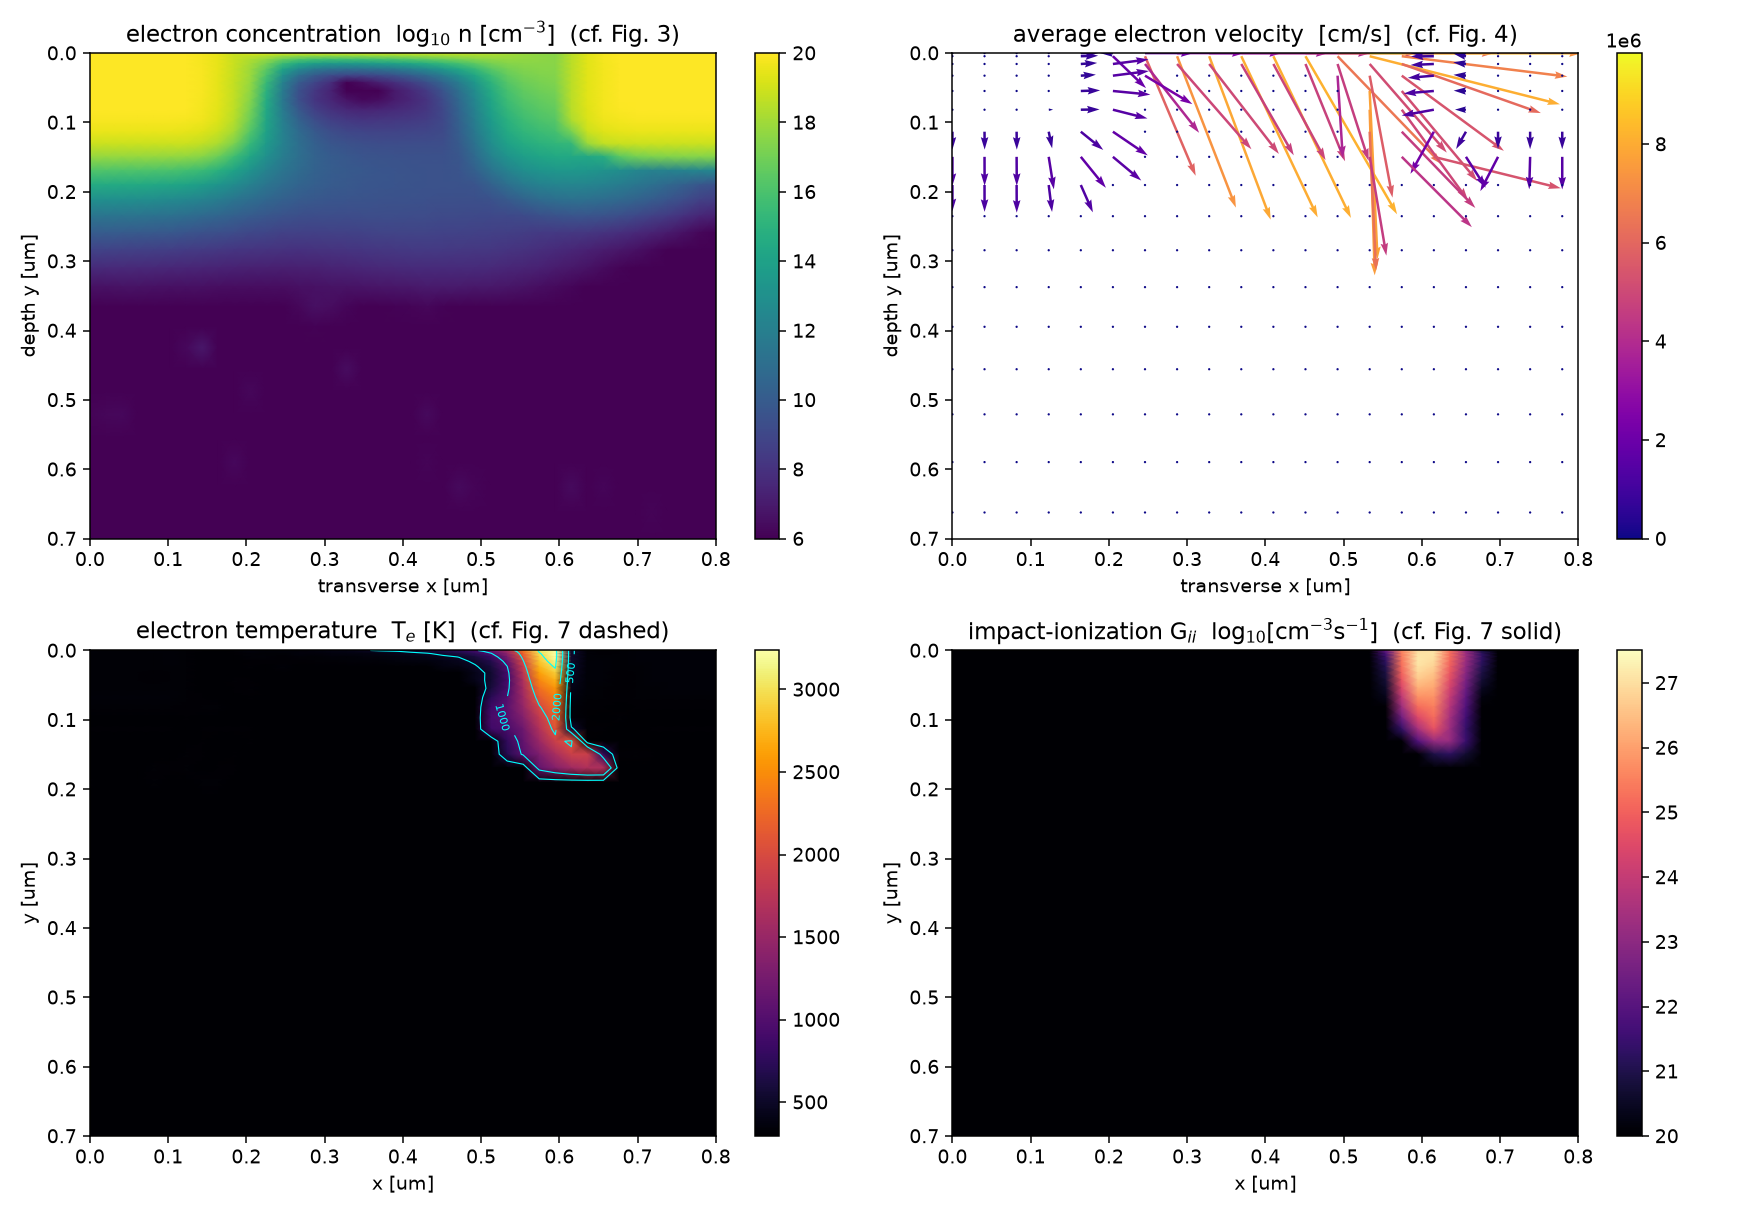
\includegraphics[width=\linewidth]{../figures/she2d_moments.png}
\caption{SHE moments at $V_{gs}=V_{ds}=\SI{3}{V}$. \textbf{Fig.~3} (top-left) electron
concentration: source/drain n$^+$ at $10^{20}$, surface inversion layer, drain-side
pinch-off. \textbf{Fig.~4} (top-right) average-velocity field: source$\to$drain flow
saturating at $\sim\!1.2\times10^7\,\si{cm/s}$ in the high-field region. \textbf{Fig.~7}
(bottom) electron temperature (peaks at the drain, \SI{3236}{K}) and impact-ionization rate
(peaks at the drain, $1.4\times10^{27}\,\si{cm^{-3}s^{-1}}$); the two peaks are
\emph{offset}, the effect Liang \emph{et al.} emphasize.}
\end{figure}

\begin{figure}[h]\centering
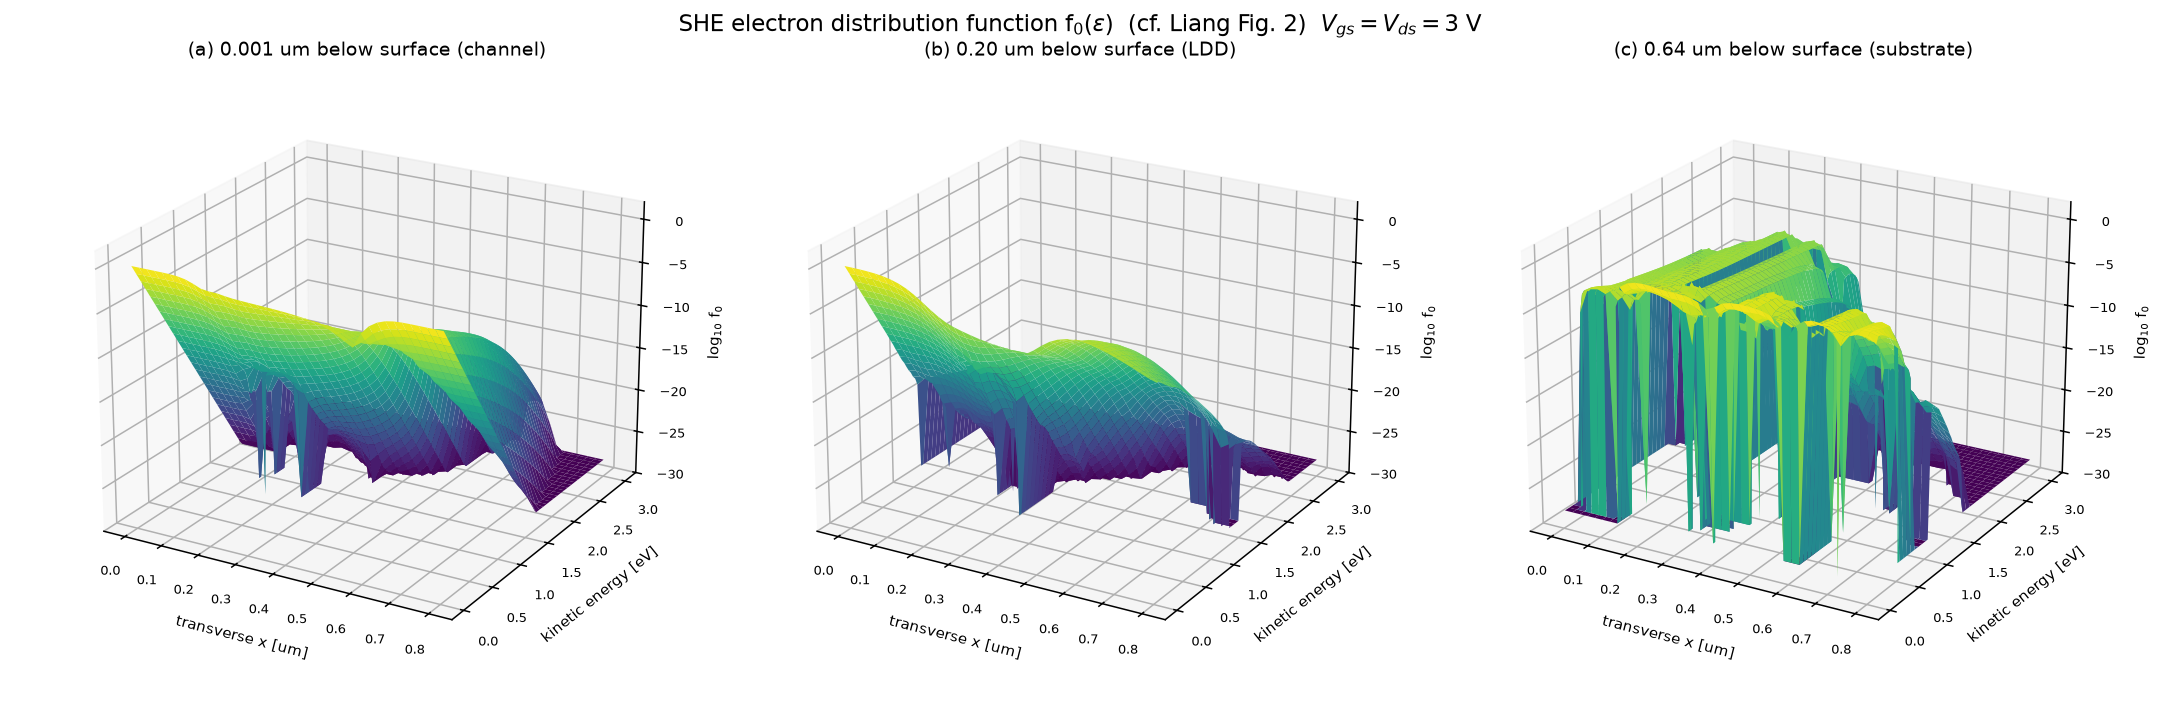
\includegraphics[width=\linewidth]{../figures/she2d_fig2_distribution.png}
\caption{\textbf{Fig.~2}: electron distribution $f_0(\eps)$ (normalized, $\log_{10}$) versus
transverse position and kinetic energy at three depths. The channel line (a) develops a
\emph{hot high-energy tail near the drain} ($x\!\sim\!0.5$--$0.6\,\si{\micro\meter}$); the
deep-substrate line (c) is essentially carrier-free (hence noisy). Hot-tail fraction
($\eps>\SI{1}{eV}$, $x=\SI{0.6}{\micro\meter}$): $5.8\times10^{-3}$ (channel) vs.\
$1.1\times10^{-8}$ (0.2\,\si{\micro\meter}).}
\end{figure}

\begin{table}[h]\centering\small
\caption{Physical validation of the SHE moments against known scales / the paper.}
\label{tab:val}
\begin{tabular}{p{5.6cm}rl}
\toprule
Quantity & Computed & Reference / paper\\
\midrule
peak electron concentration [\si{cm^{-3}}] & $1.05\times10^{20}$ & n$^+$ S/D $\sim10^{20}$ \\
peak average velocity [\si{cm/s}] & $1.23\times10^{7}$ & saturation $v_s\sim10^{7}$ \\
peak electron temperature [K] & $3236$ & Fig.~7 contours to $\sim5000$ (drain) \\
peak impact-ionization $G_{ii}$ [\si{cm^{-3}s^{-1}}] & $1.37\times10^{27}$ & Fig.~7 contours $10^{26}$--$2.3\times10^{27}$ \\
location of $T_e$ / $G_{ii}$ peaks & drain, offset & drain, offset (paper's key point) \\
distribution hot tail & channel$\gg$substrate & Fig.~2: heated near drain \\
\bottomrule
\end{tabular}
\end{table}

Every computed magnitude lands on the correct physical scale, and the spatial structure
(inversion, pinch-off, drain-localized heating and generation, source$\to$drain velocity
saturation, near-drain distribution heating) matches Liang's Figs.~2--7 qualitatively,
including the specific $T_e$/$G_{ii}$ peak offset.

\section{Honest caveats}
\begin{itemize}[leftmargin=1.4em,itemsep=1pt]
\item \textbf{One-way coupling.} The SHE runs on the \emph{DD} potential; $n_{\text{SHE}}$
is not yet fed back to Poisson. The self-consistent SHE$\leftrightarrow$Poisson$\leftrightarrow$
hole-continuity loop (paper Fig.~1) is pending.
\item \textbf{Grid.} $40\times34\times562$ with $E_{op}=4$ energy nodes is moderate; the
maps are smooth but not converged. An $E_{op}\!\ge\!8$, finer-space study is needed for
quantitative contours.
\item \textbf{Operating point.} $V_{th}=\SI{1.64}{V}$ (un-recalibrated) $\Rightarrow$ modest
overdrive; the inversion layer is thinner than the paper's. Recalibration (lower implant)
precedes a quantitative match.
\item \textbf{Fig.~2(c)} is numerical residual (the 0.64-\si{\micro\meter} depth is
carrier-free at this bias); the paper's clean Maxwellian there reflects their fuller solution.
\item \textbf{Surrogates} (Kane band, Keldysh $\tau_{ii}$, $\tau_{ac}=\tau_1$) bias the
high-energy tail and hence $G_{ii}$ quantitatively.
\end{itemize}

\section{Remaining work}
\begin{enumerate}[leftmargin=1.5em,itemsep=1pt]
\item \textbf{Fig.~5} ($\phi$) and \textbf{Fig.~6} ($p$) --- available from the DD solve;
render as 3-D surfaces.
\item \textbf{Fig.~8} (I--V) --- bias sweep, terminal current from the SHE velocity moment.
\item \textbf{Self-consistent loop} --- feed $n_{\text{SHE}}$ to Poisson, iterate to
convergence (damped Gummel).
\item \textbf{Grid refinement} + \textbf{quantitative overlay} on Liang's contour values.
\item \textbf{Device recalibration} ($V_{th}\to\SI{0.6}{V}$) for a paper-consistent bias.
\end{enumerate}

\section*{Provenance}
Git commits: \texttt{40d5929} (first working SHE core), \texttt{d0b3834} (refined + velocity
+ distribution). Python 3.13.14, NumPy 2.5.1, SciPy 1.18.0. Modules: \texttt{she2d.py}
(solver), \texttt{she2d\_figures.py} (Figs.~3/4/7), \texttt{she2d\_fig2.py} (Fig.~2). Figures
regenerated by running the modules on the cached DD operating point.

\begin{thebibliography}{9}\small
\bibitem{liang} W.~Liang, N.~Goldsman, I.~Mayergoyz, P.~J.~Oldiges, \emph{IEEE Trans.\
Electron Devices} \textbf{44}(2), 257--267, 1997.
\bibitem{gnudi} A.~Gnudi, D.~Ventura, G.~Baccarani, F.~Odeh, \emph{Solid-State Electron.}
\textbf{36}, 575, 1993.
\bibitem{jungemann} C.~Jungemann, B.~Meinerzhagen, \emph{Hierarchical Device Simulation}.
Springer, 2003.
\bibitem{sg} D.~L.~Scharfetter, H.~K.~Gummel, \emph{IEEE TED} \textbf{ED-16}, 64, 1969.
\end{thebibliography}

\end{document}
